% Created 2017-10-21 Sat 01:23
% Intended LaTeX compiler: pdflatex
\documentclass[titlepage]{article}
\usepackage[utf8]{inputenc}
\usepackage[T1]{fontenc}
\usepackage{graphicx}
\usepackage{grffile}
\usepackage{longtable}
\usepackage{wrapfig}
\usepackage{rotating}
\usepackage[normalem]{ulem}
\usepackage{amsmath}
\usepackage{textcomp}
\usepackage{amssymb}
\usepackage{capt-of}
\usepackage{hyperref}
\hypersetup{hidelinks=true}
\setlength{\parindent}{2em}
\usepackage[margin=1in]{geometry}
\author{Hu Xiaoxiang \\
U1521319A \\
EEE \\
}
\date{21 Oct, 2017 \\
}
\title{
\includegraphics[width=\textwidth]{logo_ntu_new.png} \\
[5\baselineskip] ASSIGNMENT 1 - AUDIO EQUALIZER\\
REPORT \\
[5\baselineskip]}
\hypersetup{
 pdfauthor={Hu Xiaoxiang \\
U1521319A \\
EEE \\
},
 pdftitle={
\includegraphics[width=\textwidth]{logo_ntu_new.png} \\
[5\baselineskip] ASSIGNMENT 1 - AUDIO EQUALIZER\\
REPORT \\
[5\baselineskip]},
 pdfkeywords={},
 pdfsubject={},
 pdfcreator={Emacs 25.1.1 (Org mode 9.1.2)}, 
 pdflang={English}}
\begin{document}

\maketitle
\tableofcontents

\pagenumbering{roman}
\newpage
\pagenumbering{arabic}

\section{Introduction}
\label{sec:org888dc29}
\subsection{Background}
\label{sec:org71026ec}
Equalization technique has been applied in signal processing area for a long
period. By definition, equalization is the process of adjusting the balance
between frequency components within an electronic signal. An audio equalizer
is typically used for multiple frequency controls to adjust sound tone. To be
specific, an equalizer can compensate for deficiencies in a sound pickup or
reduce extraneous sounds, such as noise. Besides, instrument clarity can be
improved through equalizer, too. For example, boosting a sounds harmonics gives
the impression of more presence and brightness and decreasing a sounds
harmonics gives the impression of a dull, less dazzling sound.
\subsection{Motivation}
\label{sec:org3b822cf}
The development of equalizer was mainly motivated by the requirement of high
quality audio output. The audio output quality of loudspeakers may not be
uniform due to size, mechanical and cost constraints, even though they are
usually designed to have a fairly uniform response across the frequency
spectrum. Therefore, the involvement of audio equalizer is necessary to
flatten this response, or to shape it according to listener preferences.

In the early years, the audio equalizer was first implemented by analog
filters. However, the proliferation of digital audio sources in recent
decades, such as the Internet and the USB, gives an opportunity to apply
digital signal processing to audio signals. Especially, there are many
advantages, which include simplification of design and verification, greater
flexibility and reliability, and significantly superior sound quality,
allowing the creation of digital equalizer that can outperform its analog
counterparts.
\subsection{Objective}
\label{sec:orga80a719}
The objective of this project is to design and simulate an digital audio
equalizer using Matlab. It includes both implementation and evaluation of
the audio equalizer. 
\subsection{Report Outline}
\label{sec:org009a8ad}
This report mainly includes the method used to implement the audio equalizer
and performance analysis based on real audio signal input. The implementation
procedure briefly explains how to use 'App Designer' in Matlab to create a
Graphical User Interface (GUI) as well as the algorithm of the FIR filter.
The focus of performance analysis is on displaying the equalizer's simulation
result and discussing the differences among various filter setting and
outcomes.
\section{Design And System Construction}
\label{sec:orgb3428cb}
The entire audio equalizer consists of 3 major blocks: audio input, digital
audio equalizer and audio output. The audio input is implemented through
Matlab's internal audioread() function. The audio output, which includes the
DAC and reconstruction filter, is built on Matlab's sound() function.

\begin{figure}[htbp]
\centering
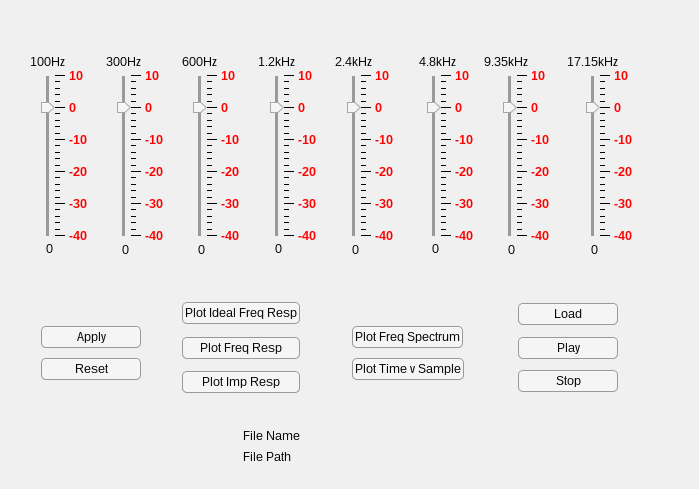
\includegraphics[width=.9\linewidth]{layout.png}
\caption{Equalizer GUI Layout}
\end{figure}

The GUI is designed by using Matlab's App Designer. As shown in Figure 1, each
frequency band in the equalizer is controlled by a slider. The 'Apply' button
collects the values of sliders and then pass them to fir2() function to
generate filters' coefficients b. The 5 'plot' buttons plot the figure of
different responses of the FIR filter, which including ideal frequency
response, actual frequency response and impulse response. The 'load' button
can let user select any audio files from their directories as filter input and
meanwhile pre-processes the input file data. The 'play' button is the
implementation of a sound() function to reconstruct the filtered data and
output analog signal. The 'stop' button is used to stop the music player.
\section{Algorithm}
\label{sec:orgb7c1253}
Function b=fir2(n,f,m,npt,lap,wind) is used to implement the multi-band filter
of this audio equalizer. n, f, m, npt, lab and wind is the representation of
filter order, frequency interval, magnitude corresponding to each frequency
interval, number of grid points, length of region around duplicate frequency
and window function respectively. Since the value of filter tap (512) is
specified, the filter order can be determined to be 511, given the formula:
\(filter order = filter tap - 1\). f the frequency range is fixed and m is
calculated by the inputs from sliders. The default value of npt and lab is
used and window function chebwin() is chosen as the input vaule of wind.

fir2 uses frequency sampling method to design FIR filter. The desired
frequency response function is interpolated linearly onto a dense, evenly
spaced grid of length npt, which is default set to 512. fir2 also sets up
regions of lap points around repeated values of f to provide steep but smooth
transitions. To obtain the filter coefficients, the function first applies an
inverse fast Fourier transform to the grid. After that, the result multiplies
by the specified window function and output the coefficients of the
numerators.

For example, to obtain the coefficients of a low pass filter like Figure 2,
the algorithm samples the desired frequency response first and then maps the
sampling points to a grid. The total number of sampling points relies on the
value of npt. Another attribute lap, as shown in Figure 3, decides the width
between two adjacent band. In other word, less the value of lab, steeper the
transitions from edge to edge. The sampling points are stored in a vector and
sent to Inverse Fast Fourier Transform (IFFT) to calculate the filter
coefficients b.

\begin{figure}[htbp]
\centering
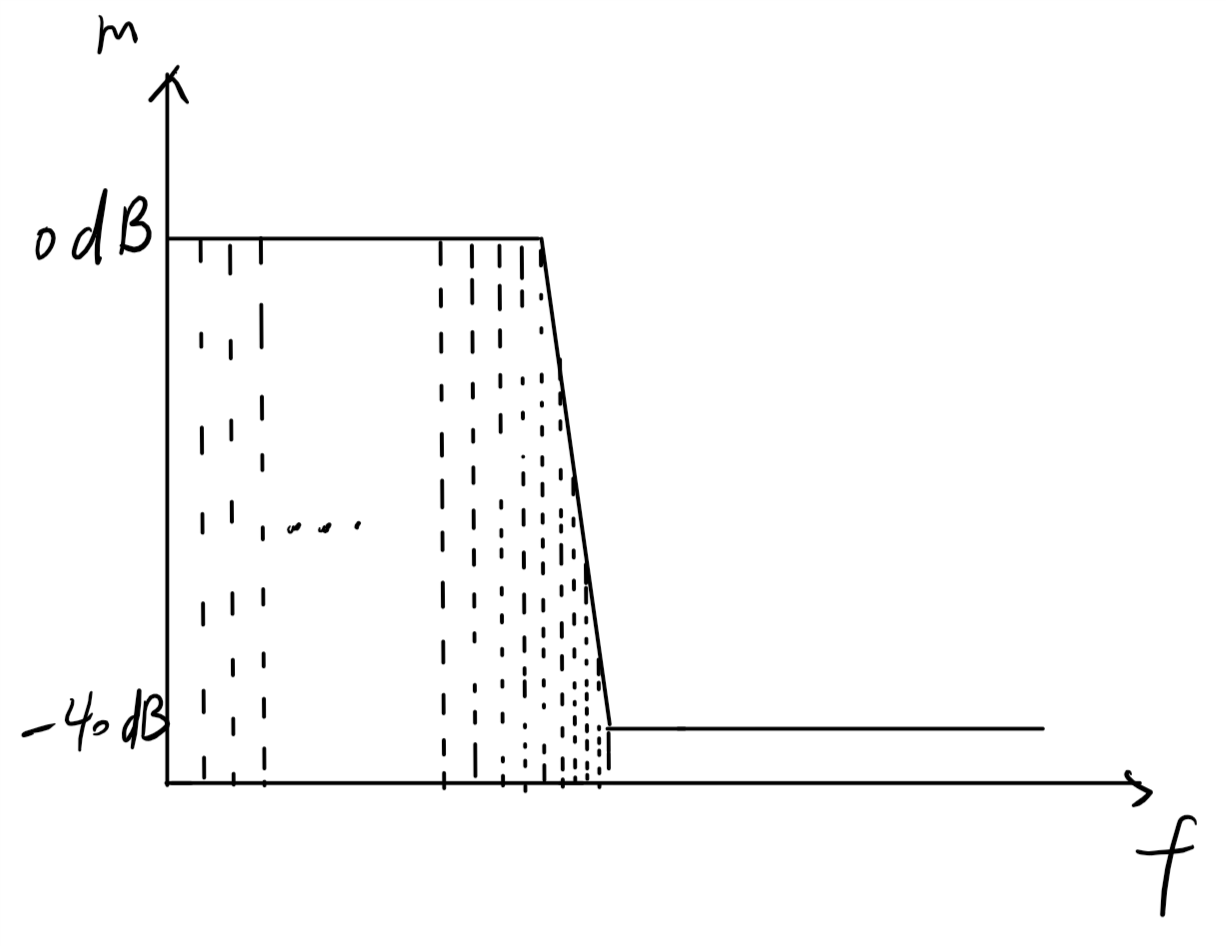
\includegraphics[width=.9\linewidth]{a.png}
\caption{Frequency Sampling}
\end{figure}
\begin{figure}[htbp]
\centering
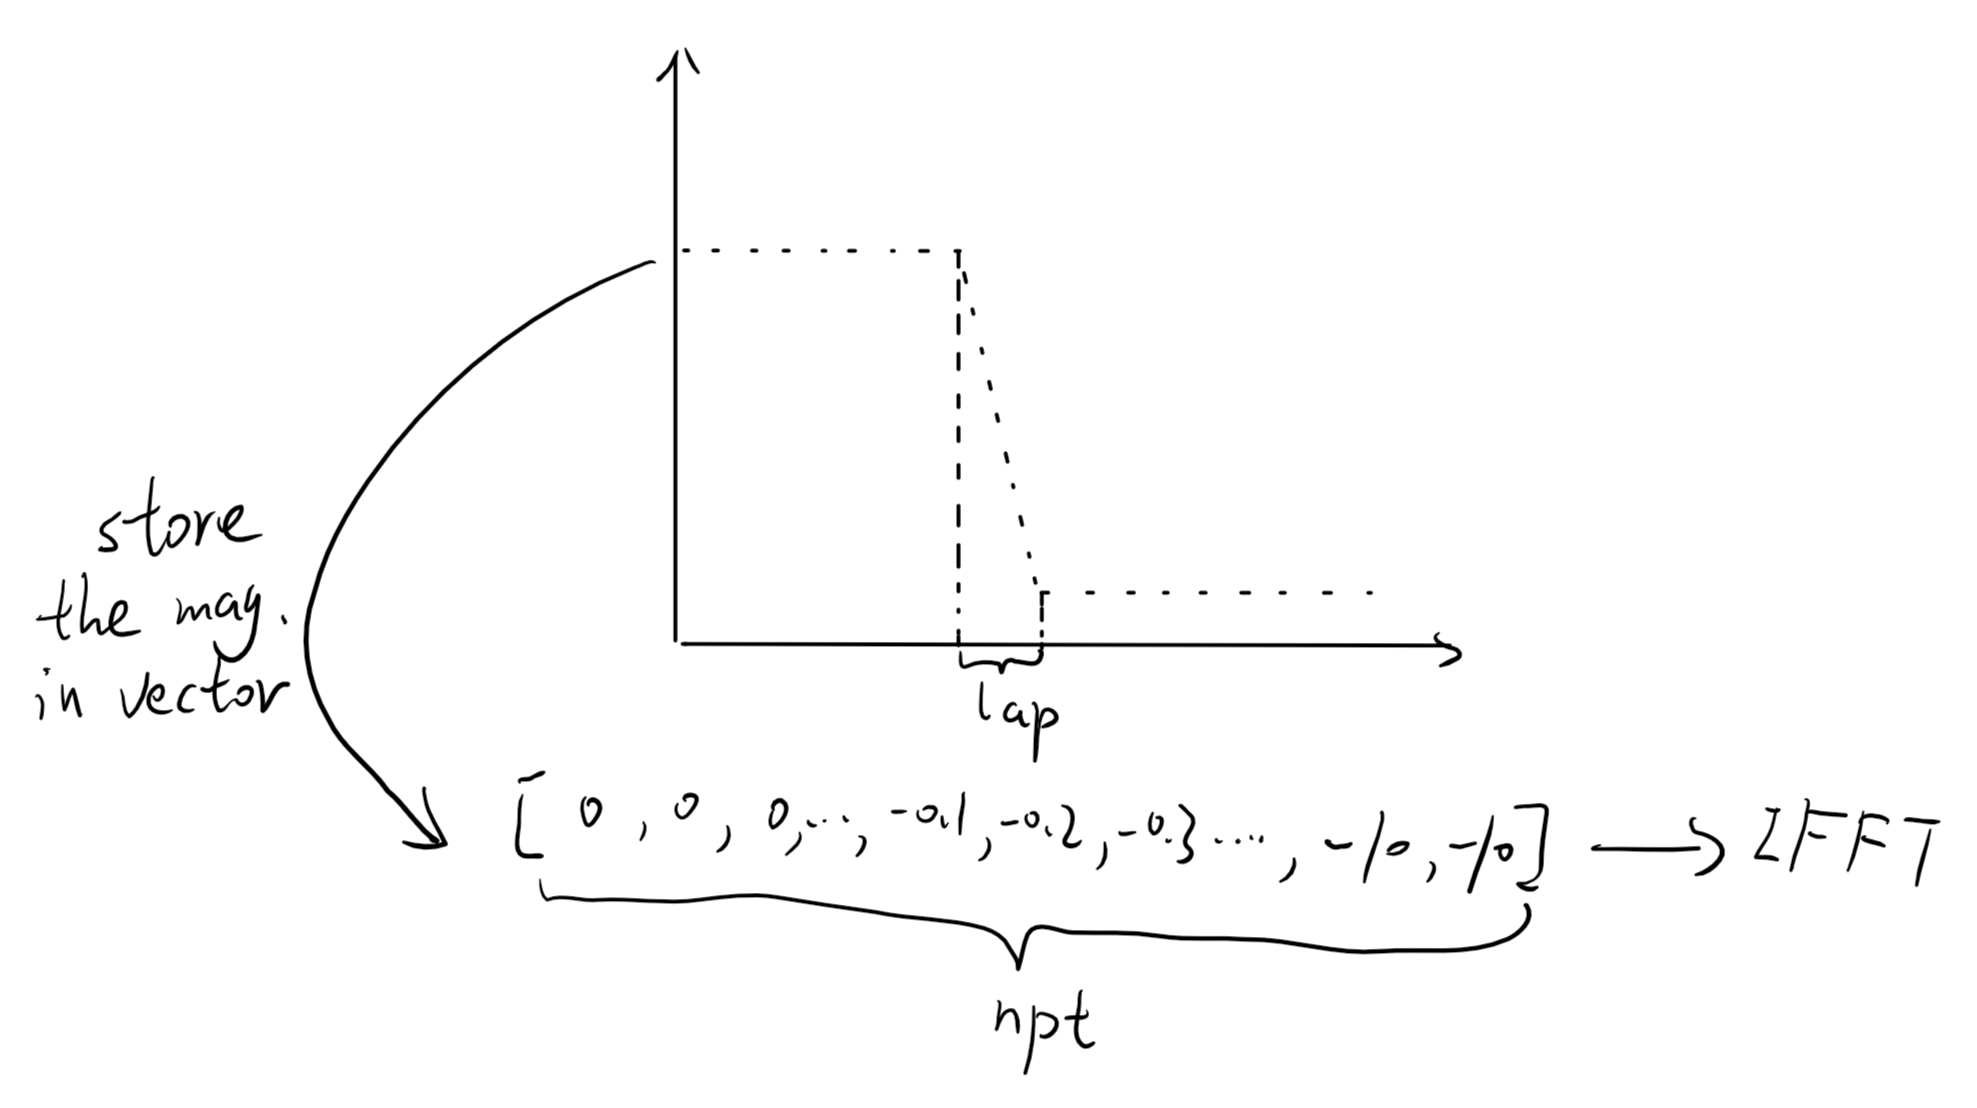
\includegraphics[width=.9\linewidth]{b.png}
\caption{Inverse Fast Fourier Transform}
\end{figure}

\section{Results And Analysis}
\label{sec:orgabfd3f8}
\subsection{Results}
\label{sec:org9c0b075}
Simulation setting: 

a) Signal components below 500 Hz and above 4000 Hz being
enhanced.

\begin{figure}[htbp]
\centering
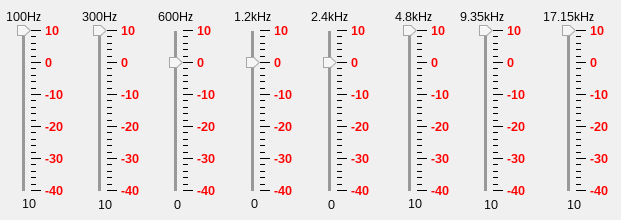
\includegraphics[width=.9\linewidth]{setting_a.png}
\caption{Setting A}
\end{figure}

\begin{figure}[htbp]
\centering
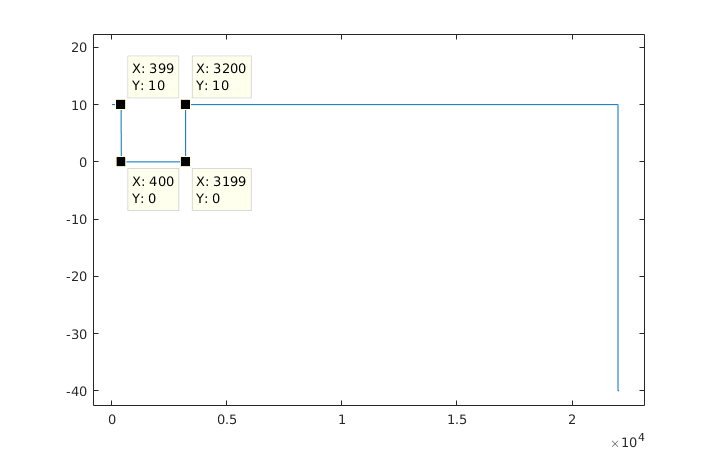
\includegraphics[width=.9\linewidth]{ideal_fr_a.png}
\caption{Ideal Frequency Response}
\end{figure}

\begin{figure}[htbp]
\centering
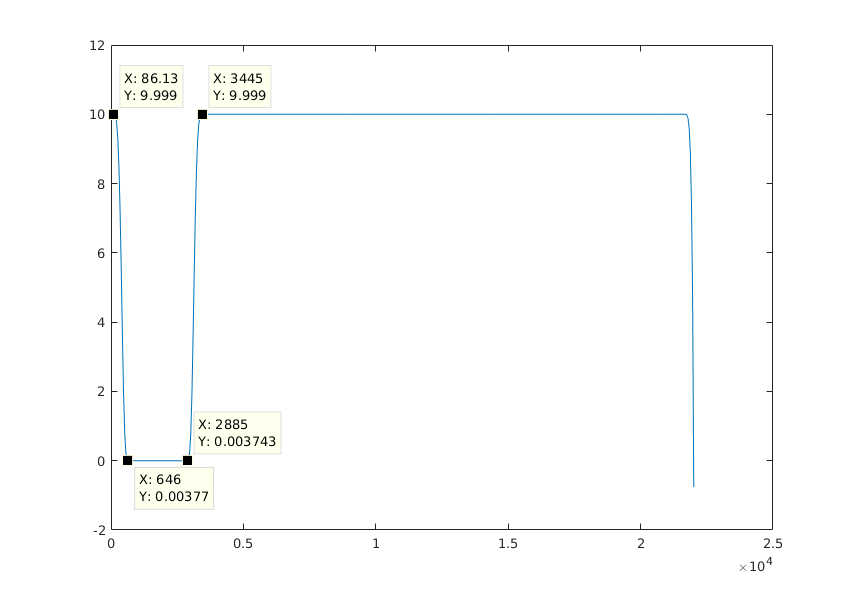
\includegraphics[width=.9\linewidth]{fr_a.png}
\caption{Actual Frequency Response}
\end{figure}

\begin{figure}[htbp]
\centering
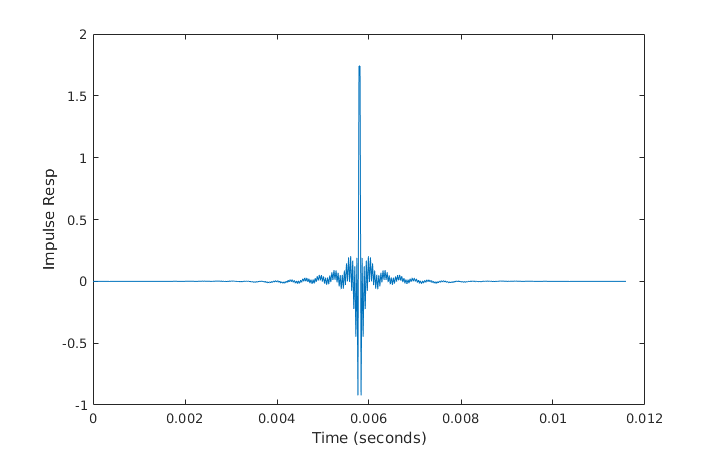
\includegraphics[width=.9\linewidth]{ir_a.png}
\caption{Impulse Response}
\end{figure}

\begin{figure}[htbp]
\centering
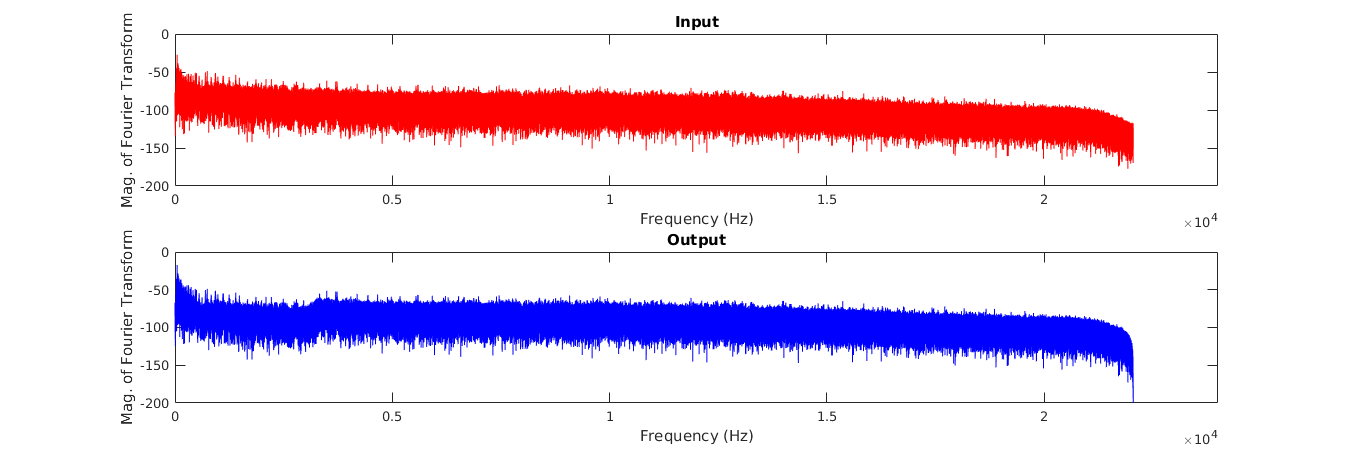
\includegraphics[width=.9\linewidth]{fs_a.png}
\caption{Frequency Spectra}
\end{figure}

\newpage  
  b) Signal components between 500 Hz and 4000 Hz being enhanced.

\begin{figure}[htbp]
\centering
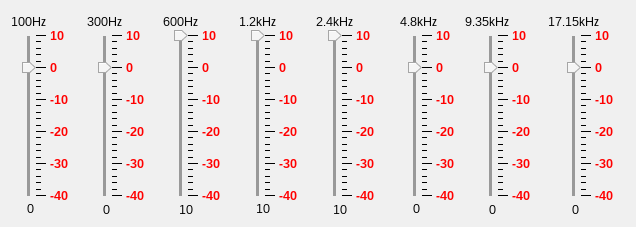
\includegraphics[width=.9\linewidth]{setting_b.png}
\caption{Setting B}
\end{figure}

\begin{figure}[htbp]
\centering
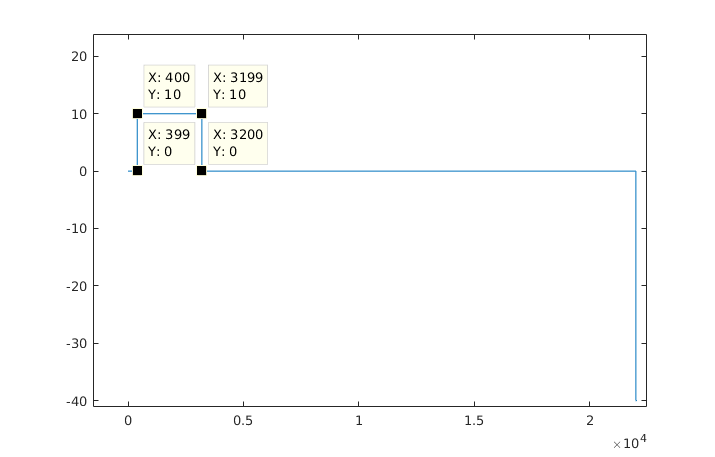
\includegraphics[width=.9\linewidth]{ideal_fr_b.png}
\caption{Ideal Frequency Response}
\end{figure}

\begin{figure}[htbp]
\centering
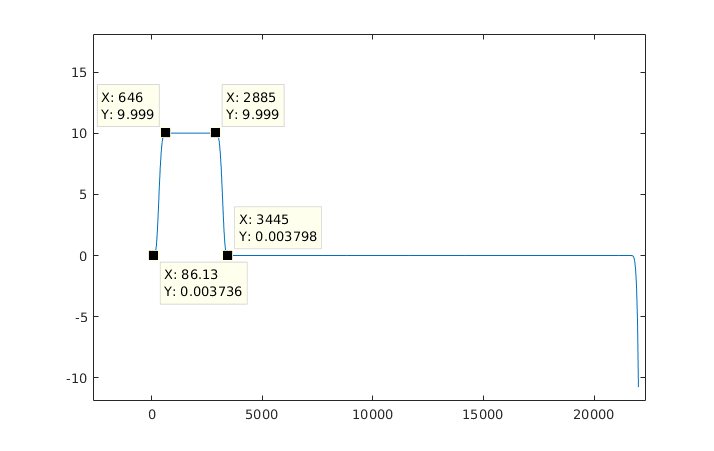
\includegraphics[width=.9\linewidth]{fr_b.png}
\caption{Actual Frequency Response}
\end{figure}

\begin{figure}[htbp]
\centering
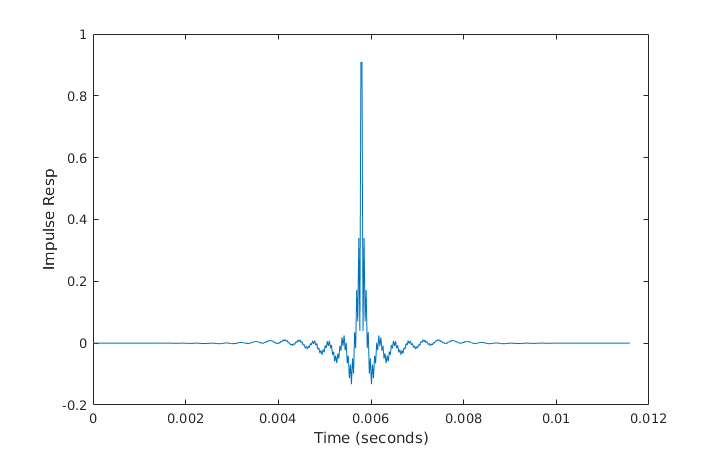
\includegraphics[width=.9\linewidth]{ir_b.png}
\caption{Impulse Response}
\end{figure}

\begin{figure}[htbp]
\centering
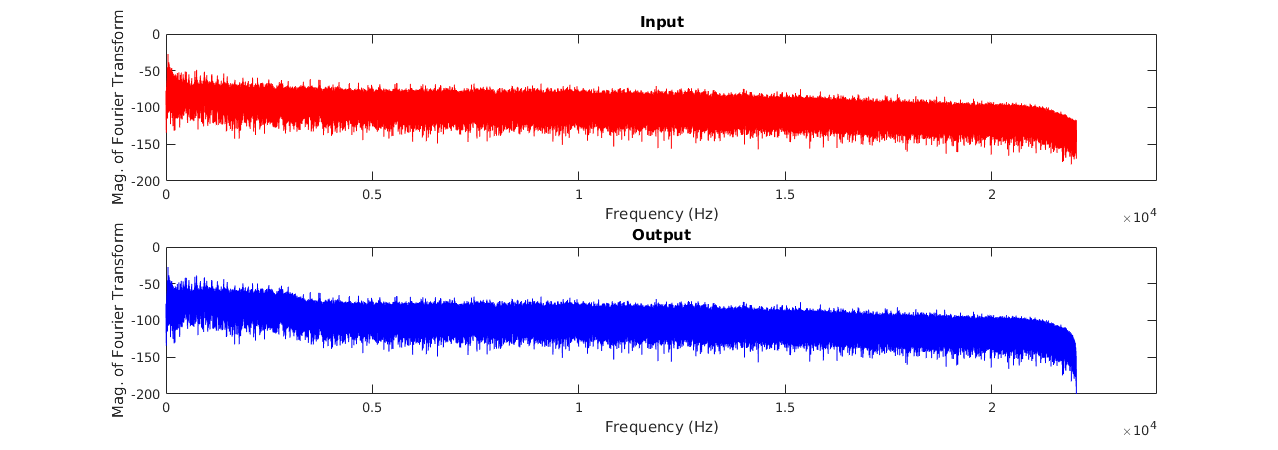
\includegraphics[width=.9\linewidth]{fs_b.png}
\caption{Frequency Spectra}
\end{figure}

\newpage
\subsection{Analysis}
\label{sec:org82a7cea}
Generally, the shape of the output frequency spectrum corresponds to the
shape of the FIR filter's frequency response. Figure 4 and 9 show two
different configurations of the equalizer. By setting the gain of band
1,2,6,7,8 to +10dB, signal components below 400 Hz and above 3200 are
enhanced. On the second configuration, where band 3,4,5 are set to +10dB,
signal components between 400 Hz and 3200 Hz are enhanced as a result.

Compared to the plot of ideal filter frequency response (Figure 5 and 10), it
is not difficult to notice that the transitions between different band edges
of actual frequency response is more smooth. The cursor on Figure 6 and 11
shows that the transition bandwidth of setting (a) is about 560 Hz, and this
is the main reason why the performance on low frequency band downgrades
significantly. Because the bandwidth of low frequency band is very narrow,
which is 200 Hz typically, a wide transition bandwidth like 560 Hz can cause
unwanted result while filtering.

To solve this problem, one way is to increase the filter order. For example,
by increasing the filter order from 511 to 800, the frequency response plot
on Figure 14 shows that the transition bandwidth reduces about 200 Hz.
However, even with the increment of filter order by almost 300, the result is
still not desirable. Actually, to design an optimized FIR filter by using
frequency sampling method, a fairly big filter order is required so as to
compensate this defect.

\begin{figure}[htbp]
\centering
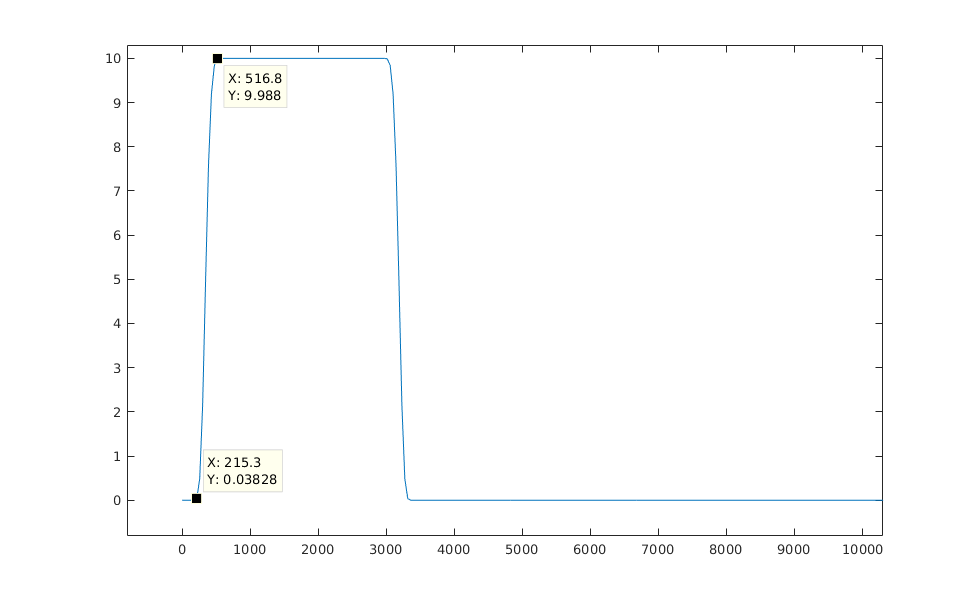
\includegraphics[width=.9\linewidth]{higher_order.png}
\caption{Frequency Response of FIR Filter with 800 Filter Order}
\end{figure}

\section{Conclusion And Recommendations}
\label{sec:org5beb6bc}
In summary, the FIR filter is able to fulfill the requirement of an audio
equalizer. The result shows that the equalizer performs better on higher
frequency band compared to lower frequency band. Generally, the frequency
sampling method is a simple way to implement FIR filter. However, this method
requires longer filter length to achieve a more precise solution. In
comparison to other design method, such as window design method, least squared
method and the Parks-McClellan method, the frequency sampling method can have
overall more error. Thus, it is recommended to implement the digital equalizer
by using other methods for a better solution on low frequency band if a higher
filter order is not allowed.

\addcontentsline{toc}{section}{References}

\begin{thebibliography}{5}

\bibitem{1} Rusty Allred and Ryan Hsiao, "The Advantages of Digital Equalization," in International IC-China, Conf., 2000

\bibitem{2}\textsc{Mathworks} (2017) fir2 
\newline
[online] Available at: https://www.mathworks.com/help/signal/ref/fir2.html

\bibitem{3}\textsc{StackExchange} (2017) Difference between frequency sampling and windowing method
\newline
[online] Available at: https://dsp.stackexchange.com/questions/31905/difference-between-frequency-sampling-and-windowing-method

\end{thebibliography}
\end{document}
